% Created by tikzDevice version 0.10.1 on 2016-08-16 16:18:04
% !TEX encoding = UTF-8 Unicode
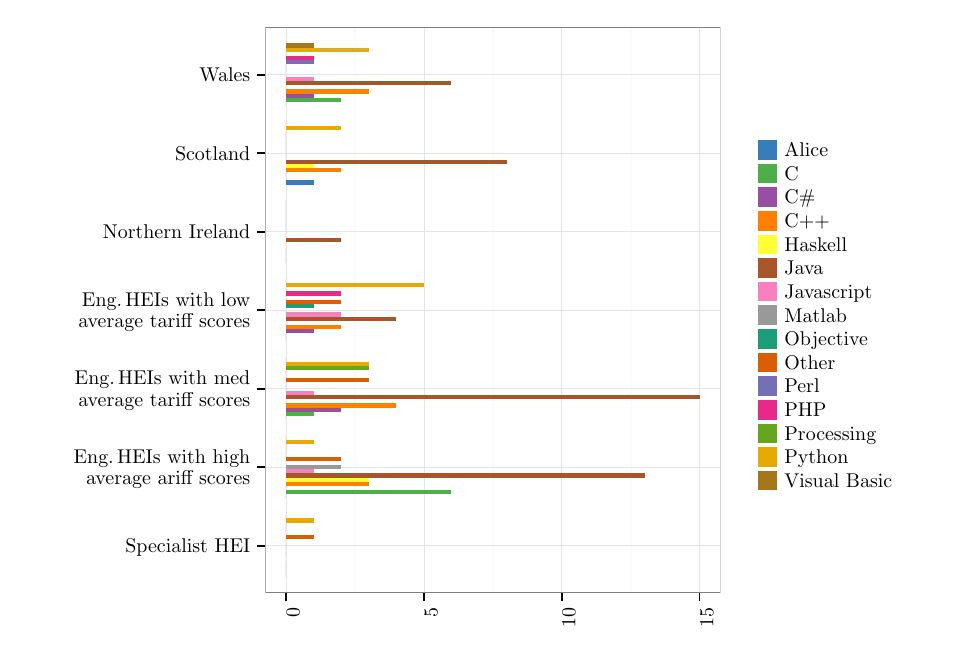
\begin{tikzpicture}[x=1pt,y=1pt]
\definecolor{fillColor}{RGB}{255,255,255}
\path[use as bounding box,fill=fillColor,fill opacity=0.00] (0,0) rectangle (325.21,216.81);
\begin{scope}
\path[clip] (  0.00,  0.00) rectangle (325.21,216.81);
\definecolor{drawColor}{RGB}{255,255,255}
\definecolor{fillColor}{RGB}{255,255,255}

\path[draw=drawColor,line width= 0.6pt,line join=round,line cap=round,fill=fillColor] (  0.00,  0.00) rectangle (325.21,216.81);
\end{scope}
\begin{scope}
\path[clip] ( 85.85, 12.60) rectangle (250.29,216.81);
\definecolor{fillColor}{RGB}{255,255,255}

\path[fill=fillColor] ( 85.85, 12.60) rectangle (250.29,216.81);
\definecolor{drawColor}{gray}{0.98}

\path[draw=drawColor,line width= 0.6pt,line join=round] (118.24, 12.60) --
	(118.24,216.81);

\path[draw=drawColor,line width= 0.6pt,line join=round] (168.07, 12.60) --
	(168.07,216.81);

\path[draw=drawColor,line width= 0.6pt,line join=round] (217.90, 12.60) --
	(217.90,216.81);
\definecolor{drawColor}{gray}{0.90}

\path[draw=drawColor,line width= 0.2pt,line join=round] ( 85.85, 29.62) --
	(250.29, 29.62);

\path[draw=drawColor,line width= 0.2pt,line join=round] ( 85.85, 57.98) --
	(250.29, 57.98);

\path[draw=drawColor,line width= 0.2pt,line join=round] ( 85.85, 86.34) --
	(250.29, 86.34);

\path[draw=drawColor,line width= 0.2pt,line join=round] ( 85.85,114.70) --
	(250.29,114.70);

\path[draw=drawColor,line width= 0.2pt,line join=round] ( 85.85,143.07) --
	(250.29,143.07);

\path[draw=drawColor,line width= 0.2pt,line join=round] ( 85.85,171.43) --
	(250.29,171.43);

\path[draw=drawColor,line width= 0.2pt,line join=round] ( 85.85,199.79) --
	(250.29,199.79);

\path[draw=drawColor,line width= 0.2pt,line join=round] ( 93.33, 12.60) --
	( 93.33,216.81);

\path[draw=drawColor,line width= 0.2pt,line join=round] (143.16, 12.60) --
	(143.16,216.81);

\path[draw=drawColor,line width= 0.2pt,line join=round] (192.99, 12.60) --
	(192.99,216.81);

\path[draw=drawColor,line width= 0.2pt,line join=round] (242.82, 12.60) --
	(242.82,216.81);
\definecolor{fillColor}{RGB}{55,126,184}

\path[fill=fillColor] ( 93.33, 18.27) rectangle ( 93.33, 19.78);
\definecolor{fillColor}{RGB}{77,175,74}

\path[fill=fillColor] ( 93.33, 19.78) rectangle ( 93.33, 21.30);
\definecolor{fillColor}{RGB}{152,78,163}

\path[fill=fillColor] ( 93.33, 21.30) rectangle ( 93.33, 22.81);
\definecolor{fillColor}{RGB}{255,127,0}

\path[fill=fillColor] ( 93.33, 22.81) rectangle ( 93.33, 24.32);
\definecolor{fillColor}{RGB}{255,255,51}

\path[fill=fillColor] ( 93.33, 24.32) rectangle ( 93.33, 25.83);
\definecolor{fillColor}{RGB}{166,86,40}

\path[fill=fillColor] ( 93.33, 25.83) rectangle ( 93.33, 27.35);
\definecolor{fillColor}{RGB}{247,129,191}

\path[fill=fillColor] ( 93.33, 27.35) rectangle ( 93.33, 28.86);
\definecolor{fillColor}{gray}{0.60}

\path[fill=fillColor] ( 93.33, 28.86) rectangle ( 93.33, 30.37);
\definecolor{fillColor}{RGB}{27,158,119}

\path[fill=fillColor] ( 93.33, 30.37) rectangle ( 93.33, 31.88);
\definecolor{fillColor}{RGB}{217,95,2}

\path[fill=fillColor] ( 93.33, 31.88) rectangle (103.29, 33.40);
\definecolor{fillColor}{RGB}{117,112,179}

\path[fill=fillColor] ( 93.33, 33.40) rectangle ( 93.33, 34.91);
\definecolor{fillColor}{RGB}{231,41,138}

\path[fill=fillColor] ( 93.33, 34.91) rectangle ( 93.33, 36.42);
\definecolor{fillColor}{RGB}{102,166,30}

\path[fill=fillColor] ( 93.33, 36.42) rectangle ( 93.33, 37.94);
\definecolor{fillColor}{RGB}{230,171,2}

\path[fill=fillColor] ( 93.33, 37.94) rectangle (103.29, 39.45);
\definecolor{fillColor}{RGB}{166,118,29}

\path[fill=fillColor] ( 93.33, 39.45) rectangle ( 93.33, 40.96);
\definecolor{fillColor}{RGB}{55,126,184}

\path[fill=fillColor] ( 93.33, 46.63) rectangle ( 93.33, 48.15);
\definecolor{fillColor}{RGB}{77,175,74}

\path[fill=fillColor] ( 93.33, 48.15) rectangle (153.12, 49.66);
\definecolor{fillColor}{RGB}{152,78,163}

\path[fill=fillColor] ( 93.33, 49.66) rectangle ( 93.33, 51.17);
\definecolor{fillColor}{RGB}{255,127,0}

\path[fill=fillColor] ( 93.33, 51.17) rectangle (123.22, 52.68);
\definecolor{fillColor}{RGB}{255,255,51}

\path[fill=fillColor] ( 93.33, 52.68) rectangle (123.22, 54.20);
\definecolor{fillColor}{RGB}{166,86,40}

\path[fill=fillColor] ( 93.33, 54.20) rectangle (222.89, 55.71);
\definecolor{fillColor}{RGB}{247,129,191}

\path[fill=fillColor] ( 93.33, 55.71) rectangle (103.29, 57.22);
\definecolor{fillColor}{gray}{0.60}

\path[fill=fillColor] ( 93.33, 57.22) rectangle (113.26, 58.73);
\definecolor{fillColor}{RGB}{27,158,119}

\path[fill=fillColor] ( 93.33, 58.73) rectangle ( 93.33, 60.25);
\definecolor{fillColor}{RGB}{217,95,2}

\path[fill=fillColor] ( 93.33, 60.25) rectangle (113.26, 61.76);
\definecolor{fillColor}{RGB}{117,112,179}

\path[fill=fillColor] ( 93.33, 61.76) rectangle ( 93.33, 63.27);
\definecolor{fillColor}{RGB}{231,41,138}

\path[fill=fillColor] ( 93.33, 63.27) rectangle ( 93.33, 64.79);
\definecolor{fillColor}{RGB}{102,166,30}

\path[fill=fillColor] ( 93.33, 64.79) rectangle ( 93.33, 66.30);
\definecolor{fillColor}{RGB}{230,171,2}

\path[fill=fillColor] ( 93.33, 66.30) rectangle (103.29, 67.81);
\definecolor{fillColor}{RGB}{166,118,29}

\path[fill=fillColor] ( 93.33, 67.81) rectangle ( 93.33, 69.32);
\definecolor{fillColor}{RGB}{55,126,184}

\path[fill=fillColor] ( 93.33, 75.00) rectangle ( 93.33, 76.51);
\definecolor{fillColor}{RGB}{77,175,74}

\path[fill=fillColor] ( 93.33, 76.51) rectangle (103.29, 78.02);
\definecolor{fillColor}{RGB}{152,78,163}

\path[fill=fillColor] ( 93.33, 78.02) rectangle (113.26, 79.53);
\definecolor{fillColor}{RGB}{255,127,0}

\path[fill=fillColor] ( 93.33, 79.53) rectangle (133.19, 81.05);
\definecolor{fillColor}{RGB}{255,255,51}

\path[fill=fillColor] ( 93.33, 81.05) rectangle ( 93.33, 82.56);
\definecolor{fillColor}{RGB}{166,86,40}

\path[fill=fillColor] ( 93.33, 82.56) rectangle (242.82, 84.07);
\definecolor{fillColor}{RGB}{247,129,191}

\path[fill=fillColor] ( 93.33, 84.07) rectangle (103.29, 85.59);
\definecolor{fillColor}{gray}{0.60}

\path[fill=fillColor] ( 93.33, 85.59) rectangle ( 93.33, 87.10);
\definecolor{fillColor}{RGB}{27,158,119}

\path[fill=fillColor] ( 93.33, 87.10) rectangle ( 93.33, 88.61);
\definecolor{fillColor}{RGB}{217,95,2}

\path[fill=fillColor] ( 93.33, 88.61) rectangle (123.22, 90.12);
\definecolor{fillColor}{RGB}{117,112,179}

\path[fill=fillColor] ( 93.33, 90.12) rectangle ( 93.33, 91.64);
\definecolor{fillColor}{RGB}{231,41,138}

\path[fill=fillColor] ( 93.33, 91.64) rectangle ( 93.33, 93.15);
\definecolor{fillColor}{RGB}{102,166,30}

\path[fill=fillColor] ( 93.33, 93.15) rectangle (123.22, 94.66);
\definecolor{fillColor}{RGB}{230,171,2}

\path[fill=fillColor] ( 93.33, 94.66) rectangle (123.22, 96.17);
\definecolor{fillColor}{RGB}{166,118,29}

\path[fill=fillColor] ( 93.33, 96.17) rectangle ( 93.33, 97.69);
\definecolor{fillColor}{RGB}{55,126,184}

\path[fill=fillColor] ( 93.33,103.36) rectangle ( 93.33,104.87);
\definecolor{fillColor}{RGB}{77,175,74}

\path[fill=fillColor] ( 93.33,104.87) rectangle ( 93.33,106.38);
\definecolor{fillColor}{RGB}{152,78,163}

\path[fill=fillColor] ( 93.33,106.38) rectangle (103.29,107.90);
\definecolor{fillColor}{RGB}{255,127,0}

\path[fill=fillColor] ( 93.33,107.90) rectangle (113.26,109.41);
\definecolor{fillColor}{RGB}{255,255,51}

\path[fill=fillColor] ( 93.33,109.41) rectangle ( 93.33,110.92);
\definecolor{fillColor}{RGB}{166,86,40}

\path[fill=fillColor] ( 93.33,110.92) rectangle (133.19,112.44);
\definecolor{fillColor}{RGB}{247,129,191}

\path[fill=fillColor] ( 93.33,112.44) rectangle (113.26,113.95);
\definecolor{fillColor}{gray}{0.60}

\path[fill=fillColor] ( 93.33,113.95) rectangle ( 93.33,115.46);
\definecolor{fillColor}{RGB}{27,158,119}

\path[fill=fillColor] ( 93.33,115.46) rectangle (103.29,116.97);
\definecolor{fillColor}{RGB}{217,95,2}

\path[fill=fillColor] ( 93.33,116.97) rectangle (113.26,118.49);
\definecolor{fillColor}{RGB}{117,112,179}

\path[fill=fillColor] ( 93.33,118.49) rectangle ( 93.33,120.00);
\definecolor{fillColor}{RGB}{231,41,138}

\path[fill=fillColor] ( 93.33,120.00) rectangle (113.26,121.51);
\definecolor{fillColor}{RGB}{102,166,30}

\path[fill=fillColor] ( 93.33,121.51) rectangle ( 93.33,123.02);
\definecolor{fillColor}{RGB}{230,171,2}

\path[fill=fillColor] ( 93.33,123.02) rectangle (143.16,124.54);
\definecolor{fillColor}{RGB}{166,118,29}

\path[fill=fillColor] ( 93.33,124.54) rectangle ( 93.33,126.05);
\definecolor{fillColor}{RGB}{55,126,184}

\path[fill=fillColor] ( 93.33,131.72) rectangle ( 93.33,133.23);
\definecolor{fillColor}{RGB}{77,175,74}

\path[fill=fillColor] ( 93.33,133.23) rectangle ( 93.33,134.75);
\definecolor{fillColor}{RGB}{152,78,163}

\path[fill=fillColor] ( 93.33,134.75) rectangle ( 93.33,136.26);
\definecolor{fillColor}{RGB}{255,127,0}

\path[fill=fillColor] ( 93.33,136.26) rectangle ( 93.33,137.77);
\definecolor{fillColor}{RGB}{255,255,51}

\path[fill=fillColor] ( 93.33,137.77) rectangle ( 93.33,139.29);
\definecolor{fillColor}{RGB}{166,86,40}

\path[fill=fillColor] ( 93.33,139.29) rectangle (113.26,140.80);
\definecolor{fillColor}{RGB}{247,129,191}

\path[fill=fillColor] ( 93.33,140.80) rectangle ( 93.33,142.31);
\definecolor{fillColor}{gray}{0.60}

\path[fill=fillColor] ( 93.33,142.31) rectangle ( 93.33,143.82);
\definecolor{fillColor}{RGB}{27,158,119}

\path[fill=fillColor] ( 93.33,143.82) rectangle ( 93.33,145.34);
\definecolor{fillColor}{RGB}{217,95,2}

\path[fill=fillColor] ( 93.33,145.34) rectangle ( 93.33,146.85);
\definecolor{fillColor}{RGB}{117,112,179}

\path[fill=fillColor] ( 93.33,146.85) rectangle ( 93.33,148.36);
\definecolor{fillColor}{RGB}{231,41,138}

\path[fill=fillColor] ( 93.33,148.36) rectangle ( 93.33,149.87);
\definecolor{fillColor}{RGB}{102,166,30}

\path[fill=fillColor] ( 93.33,149.87) rectangle ( 93.33,151.39);
\definecolor{fillColor}{RGB}{230,171,2}

\path[fill=fillColor] ( 93.33,151.39) rectangle ( 93.33,152.90);
\definecolor{fillColor}{RGB}{166,118,29}

\path[fill=fillColor] ( 93.33,152.90) rectangle ( 93.33,154.41);
\definecolor{fillColor}{RGB}{55,126,184}

\path[fill=fillColor] ( 93.33,160.08) rectangle (103.29,161.60);
\definecolor{fillColor}{RGB}{77,175,74}

\path[fill=fillColor] ( 93.33,161.60) rectangle ( 93.33,163.11);
\definecolor{fillColor}{RGB}{152,78,163}

\path[fill=fillColor] ( 93.33,163.11) rectangle ( 93.33,164.62);
\definecolor{fillColor}{RGB}{255,127,0}

\path[fill=fillColor] ( 93.33,164.62) rectangle (113.26,166.14);
\definecolor{fillColor}{RGB}{255,255,51}

\path[fill=fillColor] ( 93.33,166.14) rectangle (103.29,167.65);
\definecolor{fillColor}{RGB}{166,86,40}

\path[fill=fillColor] ( 93.33,167.65) rectangle (173.06,169.16);
\definecolor{fillColor}{RGB}{247,129,191}

\path[fill=fillColor] ( 93.33,169.16) rectangle ( 93.33,170.67);
\definecolor{fillColor}{gray}{0.60}

\path[fill=fillColor] ( 93.33,170.67) rectangle ( 93.33,172.19);
\definecolor{fillColor}{RGB}{27,158,119}

\path[fill=fillColor] ( 93.33,172.19) rectangle ( 93.33,173.70);
\definecolor{fillColor}{RGB}{217,95,2}

\path[fill=fillColor] ( 93.33,173.70) rectangle ( 93.33,175.21);
\definecolor{fillColor}{RGB}{117,112,179}

\path[fill=fillColor] ( 93.33,175.21) rectangle ( 93.33,176.72);
\definecolor{fillColor}{RGB}{231,41,138}

\path[fill=fillColor] ( 93.33,176.72) rectangle ( 93.33,178.24);
\definecolor{fillColor}{RGB}{102,166,30}

\path[fill=fillColor] ( 93.33,178.24) rectangle ( 93.33,179.75);
\definecolor{fillColor}{RGB}{230,171,2}

\path[fill=fillColor] ( 93.33,179.75) rectangle (113.26,181.26);
\definecolor{fillColor}{RGB}{166,118,29}

\path[fill=fillColor] ( 93.33,181.26) rectangle ( 93.33,182.77);
\definecolor{fillColor}{RGB}{55,126,184}

\path[fill=fillColor] ( 93.33,188.45) rectangle ( 93.33,189.96);
\definecolor{fillColor}{RGB}{77,175,74}

\path[fill=fillColor] ( 93.33,189.96) rectangle (113.26,191.47);
\definecolor{fillColor}{RGB}{152,78,163}

\path[fill=fillColor] ( 93.33,191.47) rectangle (103.29,192.99);
\definecolor{fillColor}{RGB}{255,127,0}

\path[fill=fillColor] ( 93.33,192.99) rectangle (123.22,194.50);
\definecolor{fillColor}{RGB}{255,255,51}

\path[fill=fillColor] ( 93.33,194.50) rectangle ( 93.33,196.01);
\definecolor{fillColor}{RGB}{166,86,40}

\path[fill=fillColor] ( 93.33,196.01) rectangle (153.12,197.52);
\definecolor{fillColor}{RGB}{247,129,191}

\path[fill=fillColor] ( 93.33,197.52) rectangle (103.29,199.04);
\definecolor{fillColor}{gray}{0.60}

\path[fill=fillColor] ( 93.33,199.04) rectangle ( 93.33,200.55);
\definecolor{fillColor}{RGB}{27,158,119}

\path[fill=fillColor] ( 93.33,200.55) rectangle ( 93.33,202.06);
\definecolor{fillColor}{RGB}{217,95,2}

\path[fill=fillColor] ( 93.33,202.06) rectangle ( 93.33,203.57);
\definecolor{fillColor}{RGB}{117,112,179}

\path[fill=fillColor] ( 93.33,203.57) rectangle (103.29,205.09);
\definecolor{fillColor}{RGB}{231,41,138}

\path[fill=fillColor] ( 93.33,205.09) rectangle (103.29,206.60);
\definecolor{fillColor}{RGB}{102,166,30}

\path[fill=fillColor] ( 93.33,206.60) rectangle ( 93.33,208.11);
\definecolor{fillColor}{RGB}{230,171,2}

\path[fill=fillColor] ( 93.33,208.11) rectangle (123.22,209.62);
\definecolor{fillColor}{RGB}{166,118,29}

\path[fill=fillColor] ( 93.33,209.62) rectangle (103.29,211.14);
\definecolor{drawColor}{gray}{0.50}

\path[draw=drawColor,line width= 0.6pt,line join=round,line cap=round] ( 85.85, 12.60) rectangle (250.29,216.81);
\end{scope}
\begin{scope}
\path[clip] (  0.00,  0.00) rectangle (325.21,216.81);
\definecolor{drawColor}{RGB}{0,0,0}

\node[text=drawColor,anchor=base east,inner sep=0pt, outer sep=0pt, scale=  0.72] at ( 80.45, 27.14) {Specialist HEI};

\node[text=drawColor,anchor=base east,inner sep=0pt, outer sep=0pt, scale=  0.72] at ( 80.45, 59.39) {~Eng.\,HEIs with high};

\node[text=drawColor,anchor=base east,inner sep=0pt, outer sep=0pt, scale=  0.72] at ( 80.45, 51.61) {average ariff scores};

\node[text=drawColor,anchor=base east,inner sep=0pt, outer sep=0pt, scale=  0.72] at ( 80.45, 87.75) {~Eng.\,HEIs with med};

\node[text=drawColor,anchor=base east,inner sep=0pt, outer sep=0pt, scale=  0.72] at ( 80.45, 79.97) {average tariff scores};

\node[text=drawColor,anchor=base east,inner sep=0pt, outer sep=0pt, scale=  0.72] at ( 80.45,116.11) {~Eng.\,HEIs with low};

\node[text=drawColor,anchor=base east,inner sep=0pt, outer sep=0pt, scale=  0.72] at ( 80.45,108.34) {average tariff scores};

\node[text=drawColor,anchor=base east,inner sep=0pt, outer sep=0pt, scale=  0.72] at ( 80.45,140.59) {Northern Ireland};

\node[text=drawColor,anchor=base east,inner sep=0pt, outer sep=0pt, scale=  0.72] at ( 80.45,168.95) {Scotland};

\node[text=drawColor,anchor=base east,inner sep=0pt, outer sep=0pt, scale=  0.72] at ( 80.45,197.31) {Wales};
\end{scope}
\begin{scope}
\path[clip] (  0.00,  0.00) rectangle (325.21,216.81);
\definecolor{drawColor}{RGB}{0,0,0}

\path[draw=drawColor,line width= 0.6pt,line join=round] ( 82.85, 29.62) --
	( 85.85, 29.62);

\path[draw=drawColor,line width= 0.6pt,line join=round] ( 82.85, 57.98) --
	( 85.85, 57.98);

\path[draw=drawColor,line width= 0.6pt,line join=round] ( 82.85, 86.34) --
	( 85.85, 86.34);

\path[draw=drawColor,line width= 0.6pt,line join=round] ( 82.85,114.70) --
	( 85.85,114.70);

\path[draw=drawColor,line width= 0.6pt,line join=round] ( 82.85,143.07) --
	( 85.85,143.07);

\path[draw=drawColor,line width= 0.6pt,line join=round] ( 82.85,171.43) --
	( 85.85,171.43);

\path[draw=drawColor,line width= 0.6pt,line join=round] ( 82.85,199.79) --
	( 85.85,199.79);
\end{scope}
\begin{scope}
\path[clip] (  0.00,  0.00) rectangle (325.21,216.81);
\definecolor{drawColor}{RGB}{0,0,0}

\path[draw=drawColor,line width= 0.6pt,line join=round] ( 93.33,  9.60) --
	( 93.33, 12.60);

\path[draw=drawColor,line width= 0.6pt,line join=round] (143.16,  9.60) --
	(143.16, 12.60);

\path[draw=drawColor,line width= 0.6pt,line join=round] (192.99,  9.60) --
	(192.99, 12.60);

\path[draw=drawColor,line width= 0.6pt,line join=round] (242.82,  9.60) --
	(242.82, 12.60);
\end{scope}
\begin{scope}
\path[clip] (  0.00,  0.00) rectangle (325.21,216.81);
\definecolor{drawColor}{RGB}{0,0,0}

\node[text=drawColor,rotate= 90.00,anchor=base east,inner sep=0pt, outer sep=0pt, scale=  0.72] at ( 98.28,  7.20) {0};

\node[text=drawColor,rotate= 90.00,anchor=base east,inner sep=0pt, outer sep=0pt, scale=  0.72] at (148.12,  7.20) {5};

\node[text=drawColor,rotate= 90.00,anchor=base east,inner sep=0pt, outer sep=0pt, scale=  0.72] at (197.95,  7.20) {10};

\node[text=drawColor,rotate= 90.00,anchor=base east,inner sep=0pt, outer sep=0pt, scale=  0.72] at (247.78,  7.20) {15};
\end{scope}
\begin{scope}
\path[clip] (  0.00,  0.00) rectangle (325.21,216.81);
\definecolor{fillColor}{RGB}{255,255,255}

\path[fill=fillColor] (258.83, 44.61) rectangle (316.68,184.80);
\end{scope}
\begin{scope}
\path[clip] (  0.00,  0.00) rectangle (325.21,216.81);
\definecolor{fillColor}{RGB}{55,126,184}

\path[fill=fillColor] (263.81,169.09) rectangle (270.92,176.20);
\end{scope}
\begin{scope}
\path[clip] (  0.00,  0.00) rectangle (325.21,216.81);
\definecolor{fillColor}{RGB}{77,175,74}

\path[fill=fillColor] (263.81,160.56) rectangle (270.92,167.67);
\end{scope}
\begin{scope}
\path[clip] (  0.00,  0.00) rectangle (325.21,216.81);
\definecolor{fillColor}{RGB}{152,78,163}

\path[fill=fillColor] (263.81,152.02) rectangle (270.92,159.13);
\end{scope}
\begin{scope}
\path[clip] (  0.00,  0.00) rectangle (325.21,216.81);
\definecolor{fillColor}{RGB}{255,127,0}

\path[fill=fillColor] (263.81,143.48) rectangle (270.92,150.60);
\end{scope}
\begin{scope}
\path[clip] (  0.00,  0.00) rectangle (325.21,216.81);
\definecolor{fillColor}{RGB}{255,255,51}

\path[fill=fillColor] (263.81,134.95) rectangle (270.92,142.06);
\end{scope}
\begin{scope}
\path[clip] (  0.00,  0.00) rectangle (325.21,216.81);
\definecolor{fillColor}{RGB}{166,86,40}

\path[fill=fillColor] (263.81,126.41) rectangle (270.92,133.53);
\end{scope}
\begin{scope}
\path[clip] (  0.00,  0.00) rectangle (325.21,216.81);
\definecolor{fillColor}{RGB}{247,129,191}

\path[fill=fillColor] (263.81,117.88) rectangle (270.92,124.99);
\end{scope}
\begin{scope}
\path[clip] (  0.00,  0.00) rectangle (325.21,216.81);
\definecolor{fillColor}{gray}{0.60}

\path[fill=fillColor] (263.81,109.34) rectangle (270.92,116.45);
\end{scope}
\begin{scope}
\path[clip] (  0.00,  0.00) rectangle (325.21,216.81);
\definecolor{fillColor}{RGB}{27,158,119}

\path[fill=fillColor] (263.81,100.80) rectangle (270.92,107.92);
\end{scope}
\begin{scope}
\path[clip] (  0.00,  0.00) rectangle (325.21,216.81);
\definecolor{fillColor}{RGB}{217,95,2}

\path[fill=fillColor] (263.81, 92.27) rectangle (270.92, 99.38);
\end{scope}
\begin{scope}
\path[clip] (  0.00,  0.00) rectangle (325.21,216.81);
\definecolor{fillColor}{RGB}{117,112,179}

\path[fill=fillColor] (263.81, 83.73) rectangle (270.92, 90.85);
\end{scope}
\begin{scope}
\path[clip] (  0.00,  0.00) rectangle (325.21,216.81);
\definecolor{fillColor}{RGB}{231,41,138}

\path[fill=fillColor] (263.81, 75.20) rectangle (270.92, 82.31);
\end{scope}
\begin{scope}
\path[clip] (  0.00,  0.00) rectangle (325.21,216.81);
\definecolor{fillColor}{RGB}{102,166,30}

\path[fill=fillColor] (263.81, 66.66) rectangle (270.92, 73.77);
\end{scope}
\begin{scope}
\path[clip] (  0.00,  0.00) rectangle (325.21,216.81);
\definecolor{fillColor}{RGB}{230,171,2}

\path[fill=fillColor] (263.81, 58.13) rectangle (270.92, 65.24);
\end{scope}
\begin{scope}
\path[clip] (  0.00,  0.00) rectangle (325.21,216.81);
\definecolor{fillColor}{RGB}{166,118,29}

\path[fill=fillColor] (263.81, 49.59) rectangle (270.92, 56.70);
\end{scope}
\begin{scope}
\path[clip] (  0.00,  0.00) rectangle (325.21,216.81);
\definecolor{drawColor}{RGB}{0,0,0}

\node[text=drawColor,anchor=base west,inner sep=0pt, outer sep=0pt, scale=  0.72] at (273.44,170.17) {Alice};
\end{scope}
\begin{scope}
\path[clip] (  0.00,  0.00) rectangle (325.21,216.81);
\definecolor{drawColor}{RGB}{0,0,0}

\node[text=drawColor,anchor=base west,inner sep=0pt, outer sep=0pt, scale=  0.72] at (273.44,161.63) {C};
\end{scope}
\begin{scope}
\path[clip] (  0.00,  0.00) rectangle (325.21,216.81);
\definecolor{drawColor}{RGB}{0,0,0}

\node[text=drawColor,anchor=base west,inner sep=0pt, outer sep=0pt, scale=  0.72] at (273.44,153.10) {C\#};
\end{scope}
\begin{scope}
\path[clip] (  0.00,  0.00) rectangle (325.21,216.81);
\definecolor{drawColor}{RGB}{0,0,0}

\node[text=drawColor,anchor=base west,inner sep=0pt, outer sep=0pt, scale=  0.72] at (273.44,144.56) {C++};
\end{scope}
\begin{scope}
\path[clip] (  0.00,  0.00) rectangle (325.21,216.81);
\definecolor{drawColor}{RGB}{0,0,0}

\node[text=drawColor,anchor=base west,inner sep=0pt, outer sep=0pt, scale=  0.72] at (273.44,136.03) {Haskell};
\end{scope}
\begin{scope}
\path[clip] (  0.00,  0.00) rectangle (325.21,216.81);
\definecolor{drawColor}{RGB}{0,0,0}

\node[text=drawColor,anchor=base west,inner sep=0pt, outer sep=0pt, scale=  0.72] at (273.44,127.49) {Java};
\end{scope}
\begin{scope}
\path[clip] (  0.00,  0.00) rectangle (325.21,216.81);
\definecolor{drawColor}{RGB}{0,0,0}

\node[text=drawColor,anchor=base west,inner sep=0pt, outer sep=0pt, scale=  0.72] at (273.44,118.95) {Javascript};
\end{scope}
\begin{scope}
\path[clip] (  0.00,  0.00) rectangle (325.21,216.81);
\definecolor{drawColor}{RGB}{0,0,0}

\node[text=drawColor,anchor=base west,inner sep=0pt, outer sep=0pt, scale=  0.72] at (273.44,110.42) {Matlab};
\end{scope}
\begin{scope}
\path[clip] (  0.00,  0.00) rectangle (325.21,216.81);
\definecolor{drawColor}{RGB}{0,0,0}

\node[text=drawColor,anchor=base west,inner sep=0pt, outer sep=0pt, scale=  0.72] at (273.44,101.88) {Objective};
\end{scope}
\begin{scope}
\path[clip] (  0.00,  0.00) rectangle (325.21,216.81);
\definecolor{drawColor}{RGB}{0,0,0}

\node[text=drawColor,anchor=base west,inner sep=0pt, outer sep=0pt, scale=  0.72] at (273.44, 93.35) {Other};
\end{scope}
\begin{scope}
\path[clip] (  0.00,  0.00) rectangle (325.21,216.81);
\definecolor{drawColor}{RGB}{0,0,0}

\node[text=drawColor,anchor=base west,inner sep=0pt, outer sep=0pt, scale=  0.72] at (273.44, 84.81) {Perl};
\end{scope}
\begin{scope}
\path[clip] (  0.00,  0.00) rectangle (325.21,216.81);
\definecolor{drawColor}{RGB}{0,0,0}

\node[text=drawColor,anchor=base west,inner sep=0pt, outer sep=0pt, scale=  0.72] at (273.44, 76.27) {PHP};
\end{scope}
\begin{scope}
\path[clip] (  0.00,  0.00) rectangle (325.21,216.81);
\definecolor{drawColor}{RGB}{0,0,0}

\node[text=drawColor,anchor=base west,inner sep=0pt, outer sep=0pt, scale=  0.72] at (273.44, 67.74) {Processing};
\end{scope}
\begin{scope}
\path[clip] (  0.00,  0.00) rectangle (325.21,216.81);
\definecolor{drawColor}{RGB}{0,0,0}

\node[text=drawColor,anchor=base west,inner sep=0pt, outer sep=0pt, scale=  0.72] at (273.44, 59.20) {Python};
\end{scope}
\begin{scope}
\path[clip] (  0.00,  0.00) rectangle (325.21,216.81);
\definecolor{drawColor}{RGB}{0,0,0}

\node[text=drawColor,anchor=base west,inner sep=0pt, outer sep=0pt, scale=  0.72] at (273.44, 50.67) {Visual Basic};
\end{scope}
\end{tikzpicture}
